\documentclass[11pt]{article}
\usepackage[margin=0.75in, top=0.4in, bottom=0.5in]{geometry}
\usepackage{listings}
\usepackage{xcolor}
\usepackage{enumitem}
\usepackage{amsmath}
\usepackage{tikz}
\usetikzlibrary{arrows.meta,positioning}

\lstset{
  language=Java,
  basicstyle=\ttfamily\small,
  keywordstyle=\bfseries\color{blue!70!black},
  commentstyle=\color{green!50!black},
  stringstyle=\color{red!60!black},
  showstringspaces=false,
  frame=single,
  framesep=4pt,
  xleftmargin=4pt,
  xrightmargin=4pt,
  aboveskip=6pt,
  belowskip=6pt,
}

\pagestyle{empty}

\begin{document}

\begin{center}
  {\Large \textbf{CSCI-UA 102 --- Quiz 11}} \\[4pt]
  {\large Graphs --- Directed Line Graph} \\[3pt]
  Name: \underline{\hspace{2.5in}} \quad NetID: \underline{\hspace{1.5in}}
\end{center}

\medskip

\noindent Given a directed graph $G$, its \textbf{directed line graph} $L(G)$ has one vertex for each edge of $G$. For two edges $e_1 = (a, b)$ and $e_2 = (c, d)$ in $G$, we add a directed edge from $e_1$ to $e_2$ in $L(G)$ if and only if $b = c$ --- that is, whenever $e_1$ ends where $e_2$ begins.

\medskip

\noindent\textbf{(1 point)} Draw $L(G)$ for the directed graph $G$ below.

\begin{minipage}[t]{0.30\textwidth}
  \vspace{2pt}
  \centering
  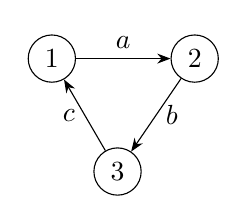
\begin{tikzpicture}[>=Stealth, vert/.style={circle, draw, minimum size=6mm, inner sep=1pt}]
    \node[vert] (v1) {1};
    \node[vert] (v2) [right=12mm of v1] {2};
    \node[vert] (v3) [below right=10mm and 4mm of v1] {3};
    \draw[->] (v1) -- node[above]{$a$} (v2);
    \draw[->] (v2) -- node[right]{$b$} (v3);
    \draw[->] (v3) -- node[left]{$c$} (v1);
  \end{tikzpicture}
\end{minipage}%
\hfill
\begin{minipage}[t]{0.65\textwidth}
  \vspace{2pt}
  \textit{Your $L(G)$:}
  \vspace{1.1in}
\end{minipage}

\medskip

\noindent\textbf{(3 points)} Write a method
\begin{center}
\texttt{static <V, E> Graph<E, V> directedLineGraph(Graph<V, E> graph)}
\end{center}
that returns the directed line graph of the input.

\smallskip

\noindent\textit{API reminder (from the course's \texttt{Graph} interface, implemented by \texttt{EdgeListGraph}):}
\begin{lstlisting}[basicstyle=\ttfamily\footnotesize, frame=none, aboveskip=2pt, belowskip=2pt, xleftmargin=8pt]
interface Graph<V, E> {                         // V = vertex elem, E = edge elem
  PositionList<Vertex<V>>   vertices();
  PositionList<Edge<E, V>>  edges();
  PositionList<Edge<E, V>>  incomingEdges(Vertex<V> v);
  PositionList<Edge<E, V>>  outgoingEdges(Vertex<V> v);
  void  insertVertex(V x);                      // returns void!
  void  insertEdge(Vertex<V> from, Vertex<V> to, E x);
}
interface Vertex<V> { V getElement(); }
interface Edge<E, V> { E getElement();  Vertex<V>[] getEndpoints(); }  // [0]=from, [1]=to
\end{lstlisting}
\textit{Tip:} since \texttt{insertVertex} returns \texttt{void}, grab the newly-added vertex via \texttt{L.vertices().last().getElement()}.

\vspace{2.7in}

\noindent\textbf{(1 point)} What is the worst-case asymptotic computational complexity of your implementation?

\vfill

\newpage

{\color{blue}
\section*{Solution}

\textbf{Part 1: drawing $L(G)$.}

\begin{center}
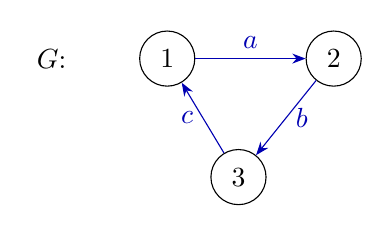
\begin{tikzpicture}[>=Stealth, vert/.style={circle, draw, minimum size=7mm, inner sep=1pt}]
  \node[vert] (v1) {1};
  \node[vert] (v2) [right=14mm of v1] {2};
  \node[vert] (v3) [below right=10mm and 4mm of v1] {3};
  \draw[color=blue!70!black, ->] (v1) -- node[above]{$a$} (v2);
  \draw[color=blue!70!black, ->] (v2) -- node[right]{$b$} (v3);
  \draw[color=blue!70!black, ->] (v3) -- node[left]{$c$} (v1);
  \node [left=8mm of v1] {$G$:};
\end{tikzpicture}
\qquad\qquad
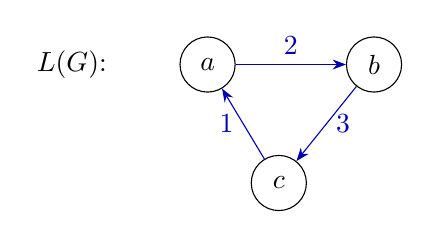
\begin{tikzpicture}[>=Stealth, vert/.style={circle, draw, minimum size=7mm, inner sep=1pt}]
  \node[vert] (a) {$a$};
  \node[vert] (b) [right=14mm of a] {$b$};
  \node[vert] (c) [below right=10mm and 4mm of a] {$c$};
  \draw[color=blue!70!black, ->] (a) -- node[above]{2} (b);
  \draw[color=blue!70!black, ->] (b) -- node[right]{3} (c);
  \draw[color=blue!70!black, ->] (c) -- node[left]{1} (a);
  \node [left=8mm of a] {$L(G)$:};
\end{tikzpicture}
\end{center}

Check each edge: $a$ ends at 2, only $b$ starts at 2 $\Rightarrow a \to b$ (shared = 2). Similarly $b \to c$ (shared = 3) and $c \to a$ (shared = 1). $L(G)$ is also a 3-cycle.

\medskip

\textbf{Part 2: Java implementation.}

\begin{lstlisting}[basicstyle=\ttfamily\small\color{blue},
  keywordstyle=\bfseries\color{blue!70!black},
  commentstyle=\color{blue!50}]
static <V, E> Graph<E, V> directedLineGraph(Graph<V, E> graph) {
    Graph<E, V> L = new EdgeListGraph<E, V>();
    Map<Edge<E, V>, Vertex<E>> edgeToVertex = new HashMapSC<>();

    // 1. one vertex in L for each edge in graph, carrying that edge's element
    for (Edge<E, V> e : graph.edges()) {
        L.insertVertex(e.getElement());
        edgeToVertex.put(e, L.vertices().last().getElement());
    }

    // 2. for each vertex v, pair its incoming edges with its outgoing edges
    //    -- each such pair is one edge in L, carrying v's element.
    for (Vertex<V> v : graph.vertices()) {
        for (Edge<E, V> e1 : graph.incomingEdges(v)) {
            for (Edge<E, V> e2 : graph.outgoingEdges(v)) {
                L.insertEdge(edgeToVertex.get(e1),
                             edgeToVertex.get(e2),
                             v.getElement());
            }
        }
    }
    return L;
}
\end{lstlisting}

\textit{Why the map?} \texttt{insertVertex} returns \texttt{void}, so after inserting we grab the just-added vertex with \texttt{L.vertices().last()} and stash it in a map keyed by the original edge. Later, when connecting two new vertices, we look them up by the corresponding pair of original edges.

\medskip

\textbf{Part 3: complexity.}

Let $n = |V(G)|$ and $m = |E(G)|$. Step~1 runs in $O(m)$.

Step~2 visits each vertex $v$ and pairs $\text{indeg}(v)$ incoming edges with $\text{outdeg}(v)$ outgoing edges. In \texttt{EdgeListGraph}, each call to \texttt{incomingEdges(v)} or \texttt{outgoingEdges(v)} scans the whole edge list, costing $O(m)$. So the outer vertex loop contributes $O(nm)$, plus $O(|E(L)|)$ inserts where $|E(L)| = \sum_v \text{indeg}(v) \cdot \text{outdeg}(v) \leq m^2$.

\smallskip

Total: $\boxed{O(nm + |E(L)|)}$ --- worst case $O(nm)$ in this representation.

\smallskip

\textit{Compared to the naive $O(m^2)$ approach} (comparing every pair of edges), this is better whenever $n < m$, which is the usual regime.

}

\end{document}
